\documentclass[conference]{sig-alternate-05-2015}
\usepackage{color, xcolor, float, lscape, enumerate, graphicx, url, tabularx, multirow, xspace, hyperref}%times
\usepackage[font=bf, skip=0pt]{caption}
\usepackage[shortlabels,inline]{enumitem}
%\usepackage{titlesec}
\usepackage[english]{babel}
\graphicspath{ {./images/} }

\hypersetup{
  colorlinks,
  citecolor=blue,
  linkcolor=red,
  urlcolor=black}
\newcommand{\note}[1]{{\textcolor{blue}{[#1]}}}
\newcommand{\fixme}[1]{{\textcolor{red}{#1}}}
\newcommand{\citeme}{{\textcolor{red}{[?]}}\xspace}
\newcommand{\todo}[1]{{\textcolor{red}{[#1]}}}
\newcommand{\BfPara}[1]{{\noindent\bf#1.}\xspace}
\newcommand{\vi}{\vspace{5mm}}
\newcommand{\etal}{{\em et al.}\xspace}
\newcommand{\eg}{{\em e.g.,}\xspace}
\newcommand{\ie}{{\em i.e.,}\xspace}
\newcommand{\etc}{{\em etc}\xspace}



\usepackage{fancyvrb}
\usepackage{verbatim}
\begin{document}



\title{Cyber-Bullying Detection and Classification System}



\author{
  Marc Mailloux\\ marcmailloux@knights.ucf.edu
  \and Rolando Nieves\\ rolando.j.nieves@knights.ucf.edu
  \and Maxim Shelopugin\\ maxim.shelopugin@knights.ucf.edu
}

\maketitle


\section{Motivation \& Problem Statement}\label{sec:motivation}
Among all the forms of bullying and harassment recognized today, bullying via
platforms hosted on the Internet has proliferated at an alarming rate. The rate
of proliferation has been concerning enough to motivate the United States
Centers for Disease Control and Prevention (CSC) to acquire and report data
regarding ``electronic'' bullying (or, as it is more commonly known,
``cyber-bullying'' via its biennial Youth Risk Behavior Surveillance System
(YRBSS) \cite{CBRC_facts2018}.

Collection of data from cyber-bullying victims has helped immensely as it
pertains to awareness and prevention. It should be possible to further improve
in both areas if data collection overcomes the limitation of the
``a posteriori'' nature of current methods (i.e., prevention methods derived
from data voluntarily disclosed by victims after harassment has occurred). An
automated system capable of examining electronic communication traffic,
identifying and classifying any traffic that could be considered as bullying,
could lead to solutions that can either filter out any offensive content
automatically, or significantly shorten the response time to an incident,
possibly preventing the more dire secondary effects of cyber-bullying.


\section{Related Work}\label{sec:related}

There has been much research done around this topic, as evidenced by the body of
work on display on the Cyber-Bullying Research Center research summary page
\cite{CBRC_research2018}. Approaches employed to date include relatively
simple Bayes type classifiers, as well as more complex deep learning systems
(Sweta Agrawal et. al. \cite{agrawal2018deep}). One existing implementation that
serves as an excellent exemplar to this proof-of-concept implementation is the
\textit{Anti Bully} project by Michelle Li \cite{Li2016}. The work documented
in this report differs from \textit{Anti Bully} in two important ways:

\begin{itemize}
  \item The implementation documented in this paper does not rely solely on
  Na\"{i}ve Bayes classification algorithms the way \textit{Anti Bully} does.
  \item The system will be able to further refine the binary
  classification done in \textit{Anti Bully} (which only identifies traffic as
  \textbf{bullying} or \textbf{not bullying}) by categorizing bullying traffic
  among one of the classes listed in Section \ref{sec:design}.
\end{itemize}

The \textit{Anti Bully} system code base does include a good data set which can
be used in the proof-of-concept documented in this paper, albeit with some
modifications (see Section \ref{sec:dataset}).

A library that has proven invaluable in the proof-of-concept implementation
documented in this paper is the \textit{Natural Language Toolkit (NLTK)}
(Bird et. al. \cite{bird2009natural}). The primary \textit{NLTK} features
leveraged in this proof-of-concept include:
\begin{itemize}
  \item Split content into sentences and words
  \item Filter out ``Stop Words'' (e.g., ``the,'' ``a,'', ``is'')
  \item ``Stemming'' (i.e., reducing words to their root)
\end{itemize}

The tutorial by Jason Brownlee titled ``How to Clean Text for Machine Learning
with Python'' \cite{brownlee-2017} was instrumental in learning how to
effectively use these \textit{NLTK} features. Indeed, the proof-of-concept
implementation documented in this paper incorporates code snippets offered in
said tutorial.

Another library that has proven very useful in this proof-of-concept
implementation, especially in the area of numerical processing, is the
\textit{TensorFlow} library produced by Google, Inc.
\cite{tensorflow2015-whitepaper}. The primary list of \textit{TensorFlow}
features used in this proof-of-concept are:
\begin{itemize}
  \item Ready-made constructs for:
  \begin{itemize}
    \item Artificial Neuron Networks (ANN)
    \item Linear and Radial Basis Function-based Support Vector Machines (SVM)
  \end{itemize}
  \item High performance parallel computing leveraging Graphical Processing
  Unit (GPU) capabilities
\end{itemize}

The design decision (as documented in Section \ref{sec:design}) regarding the
use of Comma Separated Value (CSV)-formatted files as primary input/output led
to the inclusion of the Pandas data processing library
\cite{mckinney-proc-scipy-2010}.

Finally, serving as the foundation for nearly all of these external libraries,
is the \textit{NumPy} numerical computation library \cite{oliphant2006guide}.

\section{Cyber-Bullying Detection System}\label{sec:design}
The implementation presented in this paper advocates for the implementation of a
proof-of-concept meeting the desired features as outlined in Section \ref{sec:motivation}.
Leveraging technological advances in Natural
Language Processing, along with algorithms borrowed from the areas of Artificial
Intelligence and Machine Learning, the system will be trained to recognize and
classify cyber-bullying traffic. The classification will go beyond simply
identifying bullying traffic, but will also categorize the bullying into three
(3) distinct classes:
\begin{description}
    \item[Cultural Harassment] Offensive content primarily focusing on the
    victim's race or religious beliefs.
    \item[Sexual Harassment] Amplification of stereotypical behavior for a given
    gender, or gender identification.
    \item[Personal Attacks] Ridicule based on a victim's outward-visible
    attributes, such as appearance, mannerisms, or intelligence.
\end{description}

The system, at its core, is very similar to classification systems
common in the areas of Artificial Intelligence and Machine Learning. The system
combines a classifying apparatus based on machine learning algorithms with a
natural language vector representation mechanism.

The inner workings of the system can be described as an information flow,
ultimately leading to output artifacts containing the data included in this
report. The information flows through the following set of processes (some of
which are further described in later subsections, as referenced in each list
item):
\begin{enumerate}
  \item \textbf{Pre-processing:} Accept the original input from the data set and
  prepare the data set text for feature representation (see Section
  \ref{subsec:preprocessing}).
  \item \textbf{Feature Representation:} Accept the processed input and
  transform it into vector-based feature representations (see Section
  \ref{subsec:feature_rep}).
  \item \textbf{Classification and Evaluation:} Train a classifier to predict
  labels for each of the samples in the data set, compare said predictions to
  the actual data set labels, and produce metrics describing the classification
  performance (see Section \ref{subsec:classification}). Three independent
  classifiers are used within this task:
  \begin{itemize}
    \item ANN classification - A three-layer (one input, one hidden, and
    one output) Artificial Neuron Network (ANN).
    \item SVM classification - A Radial Basis Function (RBF) Support Vector
    Machine.
    \item Bayes classification - A Na\"{i}ve Bayes classifier.
  \end{itemize}
  \item \textbf{Statistical Significance:} Determine, via statistical tests,
  which classifier(s) perform better than others (see Section
  \ref{subsec:stat_significance}).
\end{enumerate}

A simple diagram depicting the aforementioned information processing tasks, and
how information flows, is shown in Figure \ref{fig:design}.

\begin{figure}[h]
  \centering
  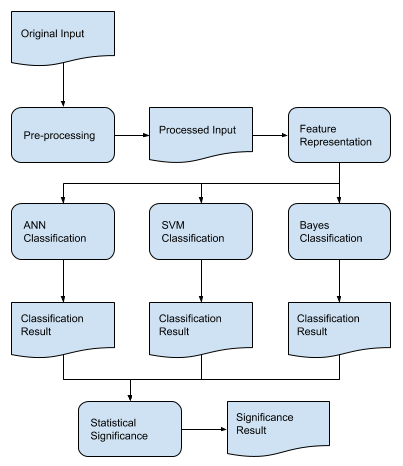
\includegraphics[width=\linewidth]{design.png}
  \caption{Flow diagram depicting the high-level design of the Cyber-bullying
  Detection and Classification System}
  \label{fig:design}
\end{figure}

In order to both save required processing time between runs, as well as capture
data that eventually is included in this report, some of these processes produce
artifacts as their resulting product. The complete list of artifacts in the
system follows:

\begin{itemize}
  \item \textbf{Original Input:} The data set as it exists prior to processing.
  \item \textbf{Processed Input:} The data set transformed by the
  \textit{Pre-processing} task (see Section \ref{subsec:processed_input}).
  \item \textbf{Classification Result:} Set of metrics that describe the
  classification performance of its corresponding classifier (see Section
  \ref{subsec:classification_result}).
  \item \textbf{Significance Result:} Statistical analysis derived from the set
  of results produced by all the system's classifiers (see Section
  \ref{subsec:stat_sig_result}).
\end{itemize}

\subsection{Pre-processing}\label{subsec:preprocessing}
The \textit{Pre-processing} process takes the original data set input and
performs the following tasks on it:

\begin{itemize}
  \item Split records and fields in the Comma Separated Values (CSV) input
  \item Replace recognized emoji character combinations with text equivalents
  \item Normalize case in the text within each data set sample
  \item Tokenize the text into words
  \item Filter out punctuation in the sample text
  \item Filter out ``stop words'' in the sample text
  \item ``Stem'' the words present in the sample text
\end{itemize}

\subsection{Processed Input}\label{subsec:processed_input}
As output, \textit{Pre-processing} creates a CSV file with a record for each
original sample, but with the sample's text portion transformed per the
aforementioned tasks.

The motivation behind having the \textit{Pre-processing} flow process produce
its output in the form of an intermediate artifact, as opposed to the more
traditional in-memory data structures, can be summed up in two points:
\begin{itemize}
  \item The time required to pre-process the data set text is not negligible,
  averaging around $15$ minutes for the whole data set.
  \item Write-compile-test cycles on the downstream processes is much more
  efficient with the pre-processor's result readily available.
  \item Downstream processes are not dependent on the \textit{Pre-processing}
  task's run time state.
\end{itemize}

\subsection{Feature Representation}\label{subsec:feature_rep}
The \textit{Feature Representation} process transforms the pre-processed sample
text into vector representations by identifying the unique 3-grams and 4-grams
present in the input, then describing each text sample as a vector expressing
the appearance frequency of these n-grams. The process is able to produce
vector representations for each text sample based on:
\begin{itemize}
  \item The presence count of unique 3-grams in the sample
  \item The presence count of unique 4-grams in the sample
  \item The concatenation of the above two results
\end{itemize}

\subsection{Classification and Evaluation}\label{subsec:classification}
As previously described, the \textit{Classification and Evaluation} process:
\begin{enumerate*}[(1)]
  \item accepts the data set after text samples have been transformed into
  vectors,
  \item uses the data set to train a classifier such that it can predict a label
  for an arbitrary sample,
  \item evaluates its predictions against the known sample labels, and
  \item produces metrics based on said evaluation.
\end{enumerate*}\par

Although the set of classifiers used in the system is quite diverse, they all
share the following design traits:
\begin{itemize}
  \item Since the data set will not contain an explicit training and test set,
  the classifiers all use 5-fold cross-validation to produce classification
  metrics.
  \item The final classification metrics are averaged over each of the
  cross-validation runs.
  \item The classifiers will produce the same set of metrics (see Section
  \ref{subsec:classification_result}).
\end{itemize}

\subsection{Classification Result}\label{subsec:classification_result}
As output, the \textit{Classification and Evaluation} process creates the
\textit{Classification Result} artifact. This artifact is a CSV-formatted file
that describes the performance of a classifier using the following metrics:
\begin{enumerate*}[(1)]
  \item Accuracy,
  \item Precision, and
  \item Recall.
\end{enumerate*}

The results produced by the individual classifiers are stored in external
artifacts in order to serve two use cases:

\begin{itemize}
  \item Import the resulting metrics easily into this report.
  \item Feed the metrics into the \textit{Statistical Significance} process.
\end{itemize}

\subsection{Statistical Significance}\label{subsec:stat_significance}
The \textit{Statistical Significance} process ingests the results from each of the
classifiers, derives a $95$\% confidence interval around the accuracy of each
classifier, and based on the confidence interval determines which (if any)
classifier is ``significantly better'' than the others. The significance test
is done by ranking the classifier accuracy scores from best to worst, then
determining whether the confidence interval of the better performers sees any
overlap with the intervals derived from the worse performing classifiers. Those
that do not exhibit an overlap with worse performers are identified as
``significantly better'' than them.

\subsection{Significance Result}\label{subsec:stat_sig_result}
The \textit{Statistical Significance} process, as its output, creates the
\textit{Significance Result} artifact. This artifact is a CSV-formatted file
that describes the $95$\% confidence interval around the accuracy score of each
classifier run. The artifact is designed for easy inclusion into this report.

\section{Evaluation}\label{sec:evaluation}

The primary focus while evaluating the system's performance will be to maximize
detection of bullying traffic (i.e., maximize true positives while minimizing
false negatives), with the minimization of otherwise innocuous traffic (i.e.,
maximizing true negatives while minimizing false positives).

Although the classifiers will produce several metrics after evaluating their
prediction performance, focusing on the \textit{Recall} classification metric
(i.e., the proportion of true positives classified properly) first and foremost
will provide a clear assessment regarding the aforementioned behavior we seek
from the system. A system that perfectly identifies all cyber bullying instances
while not misclassifying any innocuous traffic would exhibit a \textit{Recall}
score of 1.0. Although such perfect performance is likely not attainable, tuning
of the system will focus on maximizing the \textit{Recall} score.

In order to objectively evaluate the performance of all classifiers used, a
statistical significance test is done on the classifier's performance. Deriving
a $95$\% confidence interval around the \textit{Accuracy} score of each
classifier. Classifiers with a superior \textit{Accuracy} score that do not
exhibit overlap with any worse performing classifier's confidence interval are
deemed as ``significantly better.''

\subsection{Data Set}\label{sec:dataset}
The data set used in this proof-of-concept, as alluded to in Section
\ref{sec:related}, is a modified version of the data set provided by the
\textit{Anti Bully} system \cite{Li2016}. The data set as provided is labeled,
but the labels only contain two (2) classes: \textbf{bullying} and
\textbf{not bullying}. In order to meet the goals for the system as detailed in
Section \ref{sec:motivation}, the data set labeling has been
enhanced such that the samples labeled as \textbf{bullying} are distributed
among the categories identified in Section \ref{sec:design}.

\section{Expected outcomes and risk management}\label{sec:expectations}

Similar classification exercises, such as that documented by Sweta Agrawal
\cite{agrawal2018deep}, achieved an average Recall score of \( 0.87 \). Thus,
we expect this proof-of-concept to at least meet this performance baseline.

One risk tracked by the team which was eventually realized pertained to the
distribution of samples among all classes. Originally, the team identified a
risk where said distribution would be too lopsided to achieve effective
classification. A survey of the data set after completing the enhanced labeling
is shown in Table \ref{tab:dataset_survey_first}.

\begin{table}[h!]
  \centering
  \begin{tabular}{| l | r | r |}
    \hline
    Label & Count & Percentage \\
    \hline\hline
    Non-Bullying & $7,203$ & $81.7$\% \\
    \hline
    Cultural & $260$ & $2.9$\% \\
    \hline
    Sexual & $264$ & $3.0$\% \\
    \hline
    Personal & $1,090$ & $12.4$\% \\
    \hline\hline
    \textbf{TOTAL} & $8,817$ & $100.0$\% \\
    \hline
  \end{tabular}
  \caption{Data set survey immediately following enhanced labeling}
  \label{tab:dataset_survey_first}
\end{table}

As evidenced by the survey, two of the labels amount to just $3.0$\% each of the
total sample set. In order to address this extremely uneven distribution, the
team has decided to duplicate the ``Cultural'' and ``Sexual'' harassment samples
in the data set, such that the new make-up of the data set looks as shown in
Table \ref{tab:dataset_survey_final}.

\begin{table}[h!]
  \centering
  \begin{tabular}{| l | r | r |}
    \hline
    Label & Count & Percentage \\
    \hline\hline
    Non-Bullying & $7,203$ & $77.1$\% \\
    \hline
    Cultural & $520$ & $5.6$\% \\
    \hline
    Sexual & $528$ & $5.6$\% \\
    \hline
    Personal & $1,090$ & $11.7$\% \\
    \hline\hline
    \textbf{TOTAL} & $9,341$ & $100.0$\% \\
    \hline
  \end{tabular}
  \caption{Data set survey after duplication of ``Cultural'' and ``Sexual''
  harassment samples.}
  \label{tab:dataset_survey_final}
\end{table}

Improving data set diversity by lifting the class label composition percentage
floor above $5.0$\% should help suppress training-induced bias that could emerge
in classifiers due to the original lopsided class label distribution amongst
data set samples.

\section{Plan and Roles of Collaborators}\label{sec:plan_roles}
The proof-of-concept implementation exercise is divided into five (5)
primary task areas. The order in which the tasks are presented in this paper
does not necessarily represent the chronological order in which the tasks were
be carried out.

\subsection{Data Set Labeling}\label{sec:labeling_task}
As stated in Section \ref{sec:dataset}, the source data set for this
proof-of-concept needed to be refined in order to accommodate the
classification taxonomy as described in Section \ref{sec:design}. Although all
team members contributed to this task, \textbf{Mr. Marc Mailloux} serves as the
task's point of contact.

\subsection{Text Representation}\label{sec:tokenization_task}
Transforming the training and test sets from plain english into a form that the
proof-of-concept system can ingest is fundamental. For this task,
\textbf{Mr. Marc Mailloux} serves as both the primary developer and the
point of contact.

\subsection{Classifiers}\label{sec:classifier_task}
The classifier task, given its wide breadth, is divided among all team
members. A list of the classifiers that will be used, along with a short
explanation justifying their use, as well as the classifier's implementation
point of contact, follows:
\begin{itemize}
  \item Artificial Neuron Network (ANN) - ANNs possibly represent
  the most flexible of classifiers, both in the form of input they accept as
  well as the output they produce. The point of contact for this classifier is
  \textbf{Mr. Rolando Nieves}.
  \item Support Vector Machines (SVM) - SVMs have the possibility of requiring
  the least amount of computing power during both training (as compared with
  ANNs) and classification. The point of contact for this classifier will be
  \textbf{Mr. Maxim Shelopugin}.
  \item Na\"{i}ve Bayes - This was the classifier used in the \textit{Anti-Bully}
  system this proof-of-concept will be based on. It will be interesting to
  assess the impact, if any, of implementing the same classifier on a
  multi-class environment. The point of contact for this classifier will be
  \textbf{Mr. Maxim Shelopugin}.
\end{itemize}

The statistical significance testing, as described in Section
\ref{sec:evaluation}, will be implemented by \textbf{Mr. Rolando Nieves}. Mr.
Nieves will also serve as the point of contact for the classifier task.

\subsection{Presentation}\label{sec:presentation_task}
\textbf{Mr. Maxim Shelopugin} will be responsible for producing any materials
required to present the results of this proof-of-concept to interested parties,
including a summary poster.

\subsection{Final Report}\label{sec:report_task}
Although all team members will contribute content to it,
\textbf{Mr. Rolando Nieves} will be responsible for producing the final report
that will document the results observed while exercising the proof-of-concept
implementation documented in this paper.

\bibliographystyle{ieeetr}
\bibliography{milestone}


\end{document}
